\documentclass[11pt]{amsart}

\usepackage[english]{babel}
\usepackage {amsmath} 
\usepackage{amssymb}
\usepackage{amsfonts}
\usepackage{amsthm}
\usepackage{graphicx}
\usepackage[dvipsnames]{xcolor}
\usepackage{lipsum}
\usepackage[colorlinks,linkcolor=blue, citecolor=blue,urlcolor=blue]{hyperref}
\usepackage[backend=bibtex]{biblatex}
\usepackage[colorinlistoftodos]{todonotes}

\newcommand{\info}[1]{\todo[linecolor=OliveGreen,backgroundcolor=OliveGreen!25,bordercolor=OliveGreen]{#1}}
\newcommand{\unsure}[1]{\todo[linecolor=red,backgroundcolor=red!25,bordercolor=red]{#1}}
\newcommand{\change}[1]{\todo[linecolor=Plum,backgroundcolor=Plum!25,bordercolor=Plum]{#1}}

%% Environments for theorems, etc.. 
\theoremstyle{theorem} % set the style for the following theorems
\newtheorem{thm}{Theorem}[section] %\newtheorem{name}{display-text}[numbered-within]
\newtheorem{lem}[thm]{Lemma} %\newtheorem{name}[numbered-like]{display-text}
\newtheorem{cor}[thm]{Corollary}
\newtheorem{prop}[thm]{Proposition}
\newtheorem{alg}[thm]{Algorithm}
\theoremstyle{definition}       
\newtheorem{defn}[thm]{Definition}
\newtheorem{conj}[thm]{Conjecture}
\theoremstyle{example}                     
\newtheorem{prob}[thm]{Problem}
\theoremstyle{remark}                       
\newtheorem{exmp}[thm]{Example}
\newtheorem{rem}[thm]{Remark}
\newtheorem{claim}[thm]{Claim}  
\renewcommand{\theclaim}{}

\numberwithin{equation}{section}

\newcommand{\R}{\mathbb{R}}
\newcommand{\Q}{\mathbb{Q}}
\newcommand{\N}{\mathbb{N}}
\newcommand{\Z}{\mathbb{Z}}
\DeclareMathOperator{\rank}{rank}
\DeclareMathOperator{\dimension}{dim}
\DeclareMathOperator*{\supp}{supp}

\addbibresource{wavelet.bib}

\title{Introduction to Wavelets in Image Processing}
\author{Jason Ngo}
\date{2019-04-03}

\begin{document}
\maketitle

\section{Introduction}
Since the start of the 20th century, we have seen rapid development in the theory and applications of wavelets. As a mathematical tool, wavelets can be used to extract information from different kinds of data such as audio signals and images. As an attempt to explore wavelets at an introductory level, this paper will examine the first wavelet developed, called the Haar Wavelet and discuss its applications in image processing.

\vspace{8pt}
First, recall that \emph{$ L^2(\R) $} is a vector space of square integrable functions, taken with the inner product
\[ \langle f,g \rangle = \int_{\R} f(x) g(x)  dx. \]

\begin{defn} \label{haar}
	The \emph{Haar function} is the function $ \varPsi = \chi_{[0,0.5)} - \chi_{[0.5,1)} $. The \emph{Haar system} is the family
	\[ \{ \varPsi_{j,k}(x) = 2^{j/2} \varPsi (2^j x-k), \qquad j,k \in \Z \}. \]
\end{defn}

%Let $ \varPsi = \chi_{[0,0.5)} - \chi_{[0.5,1)} $ and define
%	\[ \varPsi_{j,k}(x) = 2^{j/2} \varPsi (2^j x-k), \qquad j,k \in \Z, \]
	Note that each term in the Haar system is constructed by translating and/or scaling the original $ \varPsi $ (see Figure \ref{fig:haarsystem}) and note that 
	$ \int_{\R} \varPsi(x)dx = 0 $, which makes $ \varPsi $ a wave (and in turn makes all other $ \varPsi_{j,k} $ a wave as well).
	
	\begin{figure}[h]
		\centering
		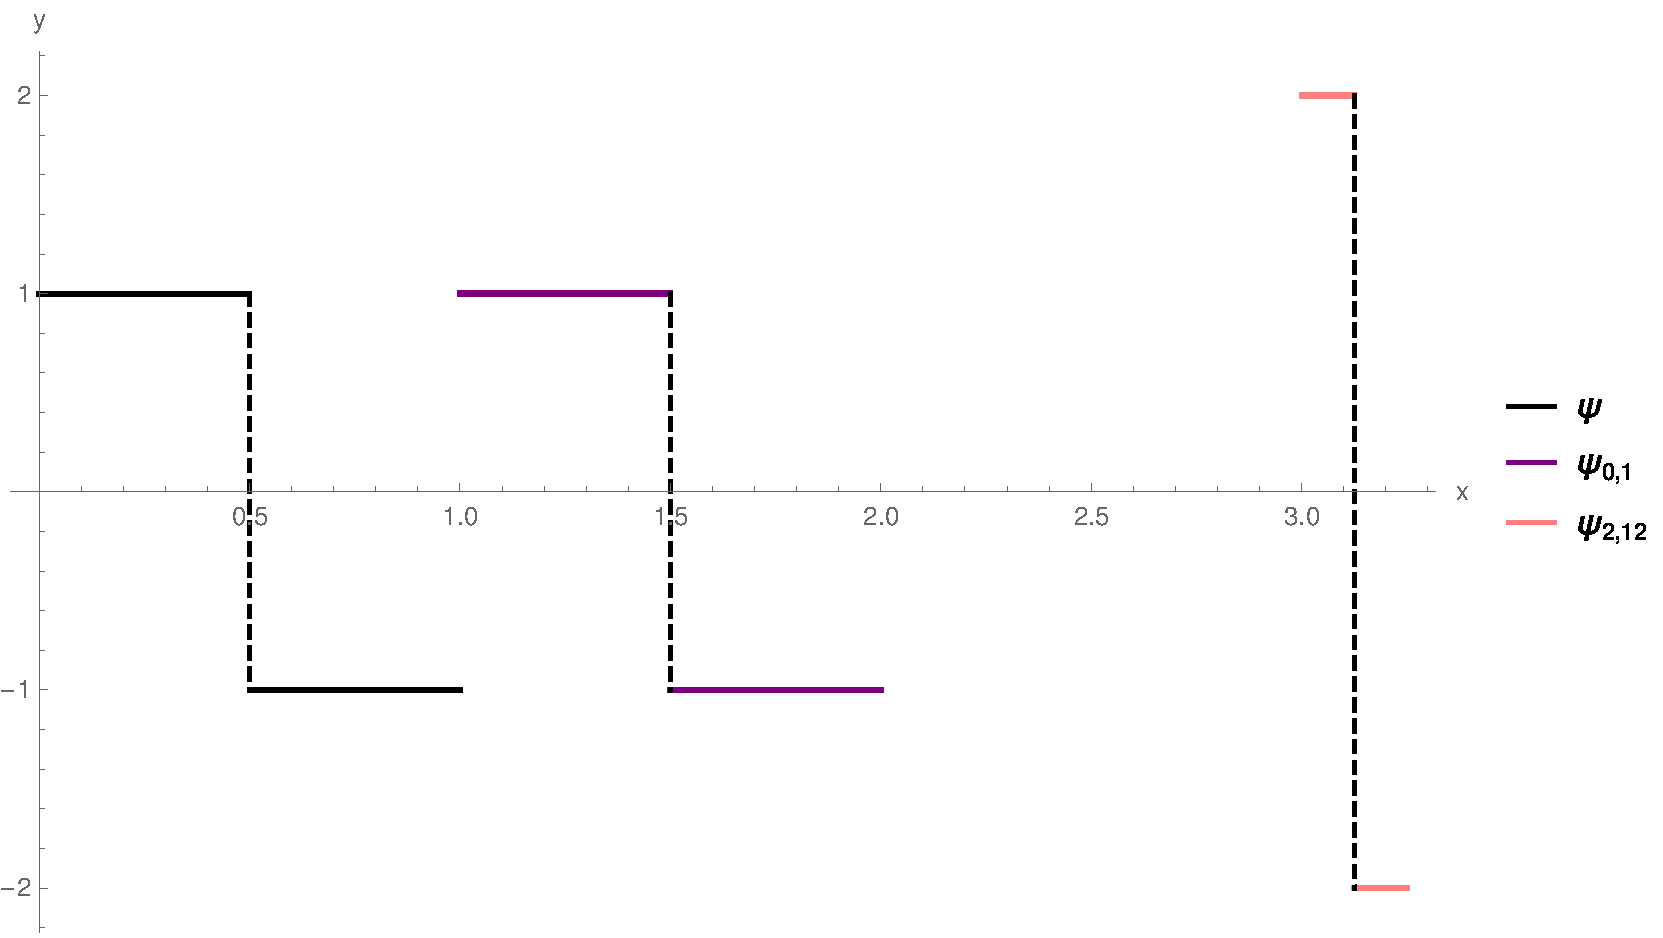
\includegraphics[width=0.7\linewidth]{img/haar_system}
		\caption[Elements of the Haar system]{Elements of the Haar system}
		\label{fig:haarsystem}
	\end{figure}
	
	We will prove that the Haar function $ \varPsi $ satisfies Definition \ref{orthonormal wavelet} of an \emph{orthonormal wavelet}.

\begin{defn}[Orthonormal Wavelet, {\cite[303]{pinsky}}] \label{orthonormal wavelet}
	
	If $ \varPsi \in L^2(\R) $, $ \varPsi_{j,k}(x) = 2^{j/2} \varPsi (2^j x-k) $, and the set $ \{ \varPsi_{j,k}: j,k \in \Z \} $ is an orthonormal basis for $ L^2(\R) $, then $ \varPsi $ is called an \emph{orthonormal wavelet}.
\end{defn}

Recall from \cite[128]{davidson} that a collection of vectors $ \{ e_n: n \in S \} $ in $ V $ is called \emph{orthonormal} if $ \|e_n\|=1 $ for all $ n \in S $ and $ \langle  e_n, e_m \rangle =0 $ for $ n \neq m \in S $. 



We have to show that the Haar system is orthonormal and spans $ L^2(\R) $.

\section{Orthonormality}
\begin{lem}[{\cite[409]{davidson}}] \label{lem:orthonormal}
	The Haar system is an orthonormal set in $ L^2(\R) $.
	
	\begin{proof}
		First, it is easy to see that $ \| \varPsi \| = 1 $. Now, let us compute:
		\begin{align*}
		\| \varPsi_{j,k} \|^2 = \int_{\R} \left| 2^{j/2} \varPsi(2^{j} x - k) \right|^2 dx 
		&=   \int_{\R} 2^j \left| \varPsi(2^{j} x - k) \right|^2 dx \\
		&= \int_{\R} \left| \varPsi(y) \right|^2 dy
		= \| \varPsi \|^2,
		\end{align*}
		by change of variable $ y = 2^{j}x-k $ in the integral. Therefore, all the elements in the Haar system has norm 1.
		
		Now, we want to show the orthogonality. Consider $ \varPsi_{j,k} $ and $ \varPsi_{j,k'} $, for $ k \neq k' $. Since these two elements have disjoint support\footnote{The \emph{support} of a function, denoted $ \supp $, is the subset of the domain containing those elements which are not mapped to zero.}, their inner product is 0. If $ j < j' $, then either $ \varPsi_{j,k} $ and $ \varPsi_{j',k'} $ have disjoint supports (when $ k \neq k' $), or supp $ \varPsi_{j',k'} $ is contained in an interval on which $ \varPsi_{j,k} $ is constant (when $ k = k' $). For the latter case, we have:
		\[ \langle \varPsi_{j,k}, \varPsi_{j',k'} \rangle = 2^j \int_{\R} \varPsi_{j',k'} dx = 0. \]
	
		Hence, the set is orthonormal.
	\end{proof}
\end{lem}

\section{Integral Kernel/Inner Product Expansion}
Now that we have proved the Haar system is orthonormal, our goal now is to show that it spans all of $ L^2(\R) $\unsure{Does the definition of span in Hilbert space means convergence? Is it the same as in Linear Algebra?}. Motivated by \cite[3]{bell} and \cite[516]{davidson}, this section will set up the integral kernel $ P_nf $ below, which will act as the foundation to prove that any function in $ L^2(\R) $ is in the span of $ \{ \varPsi_{j,k} \} $. 

\vspace{8pt}
Set $ \phi(x) = \chi_{[0,1)}$. For $ n \in \Z $, we define
\[ K_n (x,y) = 2^n \sum_{k \in \Z} \phi(2^n x - k) \phi(2^n y - k). \]

Note that $ K_n $ is either equal to $ 2^n $ (when there is some $ k \in \Z $ s.t. $ 2^n x-k $ and $ 2^ny - k $ lie in $ [0,1) $) or equal to 0 (otherwise). Equivalently, if $ K_n = 2^n $, there is some $ k $ s.t.
	\[ x,y \in \left[ \frac{k}{2^n}, \frac{k+1}{2^n} \right) = I_{n,k}. \]
Here, note that for any given $ n \in \Z $, the set $ \{ I_{n,k} \} $ is disjoint.

\info{mention something about being constant on each dyadic interval.}

We define
\[ P_n f(x) = \int_{\R} K_n(x,y) f(y) dy. \]
If $ x \in \R $ then there is a unique $ k_x \in \Z $ with $ x \in I_{n, k_x} $ and
\[ P_n f(x) = 2^n \int_{I_{n,k_x}} f(y) dy. \]

\section{Haar Wavelet Basis for $ L^2(\R) $}
\begin{lem}[{\cite[293]{pinsky}}]
	If $ n \in \Z $, then
	\[ K_{n+1} - K_n = \sum_{k \in \Z} \varPsi_{n,k}(x) \varPsi_{n,k}(y),\qquad x,y \in \R. \]
	
	\begin{proof}
		\change{The proof here is a direct copy of the proof in Bell}
		$ \varPsi(2^nx-k) = 1 $ means that $ 0 \leq 2^nx-k < \frac{1}{2} $, which is equivalent to $ \frac{2k}{2^{n+1}} \leq x < \frac{2k+1}{2^{n+1}} $, which is equivalent to $ x \in I_{n+1,2k} $. By the same argument, we have:
		\[
		\varPsi_{n,k}(x) \varPsi_{n,k} (y) =
		\begin{cases}
		2^n &\text{if} \\
		-2^n &\text{if} \\
		0 &\text{otherwise}.
		\end{cases}
		\]
		
		By our construction of $ K_n $, for the first line, indeed
		\[ K_{n+1}(x,y) - K_n(x,y) = 2^{n+1} - 2^n = 2^n \]
		
		For the second case,
		\[ K_{n+1}(x,y) - K_n(x,y) = 0 - 2^n = -2^n \]
		
		Otherwise, everything is 0.
		
		Hence, it follows that $ K_{n+1} - K_n = \sum_{k \in \Z} \varPsi_{n,k}(x) \varPsi_{n,k}(y) $.
	\end{proof}
\end{lem}

One important thing that this lemme does is to get rid of the scaling function and write integral kernel as the sum of the product of two functions from the Haar system.

\begin{rem}
	From this lemma, we also get
	\begin{align*}
		(P_{n+1} - P_n) f(x) &= \int_{\R} K_{n+1}(x,y)f(y)dy - \int_{\R} K_{n}(x,y)f(y)dy \\
		&= \int_{\R} \sum_{k \in \Z} \varPsi_{n,k}(x) \varPsi_{n,k}(y) f(y) dy \\
		&= \sum_{k \in \Z} \varPsi_{n,k}(x) \int_{\R} \varPsi_{n,k}(y) f(y) dy \\
		&= \sum_{k \in \Z} \langle f, \varPsi_{n,k} \rangle \varPsi_{n,k}(x).
	\end{align*}
	Damn, we just wrote something dependent on the scaling function entirely on the wavelet series.
	
	We call $ \langle \rangle $ the Haar coefficients.
\end{rem}

\begin{lem}[Convergence of Inner Product Expansion, {\cite[7]{bell}, \cite[517]{davidson}}]
	If $ f \in C_c(\R) $, then $ P_nf \to f $ in the uniform nom as well as in the $ L^2 $ norm.
	
	\info{draw a picture of $ P_nf $}
	\begin{proof}
		Suppose $ f \in C_c(\R) $ and $ \supp(f) \subset [-2^M, 2^M] $ for $ M \geq 0 $. Since $ f $ is continuous on a compact set, it is uniformly continuous.
		
		Given $ \epsilon > 0 $. By uniform continuity, there exists $ \delta > 0 $ such that if $ |x-y| < \delta $, then $ |f(x) - f(y)| < \epsilon $.
		
		Now, choose $ N $ such that $ 2^{-N} < \delta $; if $ n > N $, then we have:
		\begin{align*}
			|P_nf(x) - f(x)| &= \left| 2^n \int_{I_{n,k_x}} f(y)dy - f(x) \right| \\
			&=  \left| 2^n \int_{I_{n,k_x}} f(y)dy - 2^n \int_{I_{n,k_x}} f(x) dy \right| \\
			&\leq 2^n \int_{I_{n,k_x}} |f(y) - f(x)| dy\\
			&< 2^n \int_{I_{n,k_x}} \epsilon dy = \epsilon.
		\end{align*}
		Therefore, $ P_nf $ converges to $ f $ uniformly. Furthermore,
		\begin{align*}
			\| P_nf - f \|_2^2 &= \int_{\R} |P_nf(x) - f(x)|^2dx \\
			&= \int_{-2^M}^{2^M} |P_nf(x) - f(x)|^2dx \\
			&\leq \int_{-2^M}^{2^M} \|P_nf - f\|_\infty^2dx = 2 \cdot 2^M \| P_n - f \|_\infty^2.
		\end{align*}
		Since the right hand side converges to 0, by limit comparison test, it follows that $ \| P_nf-f \|_2^2 \to 0 $ as $ n \to \infty $.
		
		Hence, $ P_n \to f $ both in the uniform norm and in the $ L^2 $ norm.
	\end{proof}
\end{lem}

\info{what if the continuity hypothesis is violated mildly?}

\info{draw a picture of $ P_nf $ and $ f $ with different $ n $}

\info{what is the definition of span}
\begin{thm}[{\cite[411]{davidson}}] \label{span}
	The Haar system spans all of $ L^2(\R) $.
	
	\begin{proof}
		Let $ f $ be arbitrary in $ \in L^2(\R) $. Given $ \epsilon > 0 $.
		
		Since $ C_c(\R) $ is dense in $ L^2(\R) $\footnote{The proof for this claim can be found in \cite[326]{farrell}}, there exists $ g \in C_c(\R) $ s.t. $ |f - g| <  $
		
		\begin{align*}
			\|P_nf - f\|_2 &\leq \|P_nf - P_ng\|_2 + \|P_ng - g\|_2 + \|g - f\|_2 \\
			&\leq 
		\end{align*}
	\end{proof}
\end{thm}

Therefore, the Haar function is indeed an orthonormal wavelet. We will now refer to the Haar function as the \emph{Haar wavelet}.



\begin{exmp}
	Consider $ f(x) = e^{-x} \sin 2\pi x $ for $ x \in (0,1) $.
	
	See Figure \ref{fig:approximations} 
\end{exmp}

\section{Application to Image Processing}
 When compressing images, we want to discard the least significant details, keeping the original picture largely intact. Fortunately, wavelets can isolate and decompose a signal into low frequency part and high frequency part.
 Briefly discuss FBI Fingerprint Image Compression if there is space:
 \begin{quote}
 	 Wavelet compression methods do not require dividing the image into smaller blocks because the desired localization properties are naturally built into the wavelet system.\cite{frazier}
 \end{quote}

\printbibliography

\end{document}

